\section{Hash Map}
\begin{figure}[H]
        \centerline{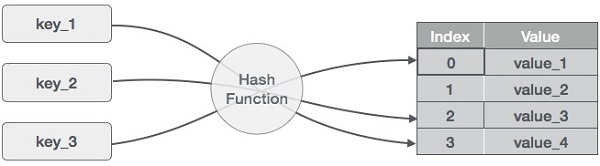
\includegraphics[scale=0.5]{figures/hash-tables/hash-function}}
        \caption{Hash Function}
\end{figure}
Dalam komputasi, tabel hash (hash map) adalah struktur data yang mengimplementasikan tipe data abstrak array asosiatif, struktur yang dapat memetakan kunci ke nilai. Tabel hash menggunakan fungsi hash untuk menghitung indeks, juga disebut kode hash, ke dalam array atau slot, dimana nilai yang diinginkan dapat ditemukan. Selama pencarian, key akan di-hash dan hash yang dihasilkan akan menunjukkan di mana nilai yang disimpan berdasarkan hash dari key. Idealnya, fungsi hash akan menetapkan setiap key ke wadah yang unik, tetapi sebagian besar desain tabel hash menggunakan fungsi hash yang tidak sempurna, yang dapat menyebabkan tabrakan hash di mana fungsi hash menghasilkan indeks yang sama untuk lebih dari satu kunci. Tabrakan seperti itu biasanya diakomodasi dalam beberapa cara. Dalam tabel hash berdimensi baik, biaya rata-rata (jumlah instruksi) untuk setiap pencarian tidak tergantung pada jumlah elemen yang disimpan dalam tabel. Banyak desain tabel hash juga memungkinkan penyisipan dan penghapusan pasangan kunci-nilai sewenang-wenang, dengan biaya rata-rata konstan (diamortisasi) per operasi. Dalam banyak situasi, tabel hash ternyata rata-rata lebih efisien daripada pohon pencarian atau struktur pencarian tabel lainnya. Untuk alasan ini, mereka banyak digunakan di berbagai jenis perangkat lunak komputer, terutama untuk array asosiatif, pengindeksan basis data, cache, dan set.

Hash Map merupakan struktur data yang memiliki indeks. Hash map menggunakan fungsi hash untuk menghitung indeks dengan key ke dalam buckets atau slot. Nilainya dipetakan ke buckets dengan indeks yang sesuai dan key yang unik dan tidak berubah. Kita ibaratkan has map dengan sebuah lemari yang memiliki laci dengan label untuk barang-barang yang disimpan di dalamnya. Misalnya, menyimpan infoemasi pengguna dan email sebagai keynya, dan kita dapat memetakan nilai yang terkait dengan pengguna tersebut seperti nama depan, nama belakang, dll ke dalam buckets.

Hashmap adalah tipe struktur data yang memetakan kunci ke pasangan nilainya (menerapkan tipe data array abstrak). Ini pada dasarnya menggunakan fungsi yang menghitung nilai indeks yang pada gilirannya menyimpan elemen yang akan dicari, dimasukkan, dihapus, dll. Ini membuatnya mudah dan cepat untuk mengakses data. Secara umum, tabel hash menyimpan pasangan key value dan key tersebut dihasilkan menggunakan fungsi hash. Jadi fungsi pencarian dan penyisipan elemen data menjadi lebih cepat karena nilai key itu sendiri menjadi indeks yang menyimpan data.

Fungsi hash adalah inti dari implementasi hash map. Fungsi hash mengambil kunci dan menerjemahkannya ke indeks buckets di daftar buckets. Hashing yang ideal harus menghasilkan indeks yang berbeda untuk setiap key. Namun, hal ini bisa menyebabkan collisions. Saat hashing memberikan indeks yang ada, kita cukup menggunakan buckets untuk beberapa nilai dengan appending list atau dengan rehashing.

Dalam python, dict merupakan contoh dari hash map. Kita akan melihat implementasi hash map dari awal untuk mempelajari cara membangun dan menyesuaikan struktur data tersebut agar dapat mengoptimalkan pencarian.
Desain hash map akan mencakup fungsi-fungsi berikut:
\begin{enumerate}

\item set\_val(key, value): Menyisipkan pasangan key-value ke dalam peta hash. Jika nilai sudah ada di peta hash, perbarui nilainya.

\item get\_val(key): Mengembalikan nilai di mana key yang ditentukan dimapping, atau “Tidak ada catatan yang ditemukan” jika map ini tidak berisi pemetaan untuk key tersebut.

\item delete\_val(key): Menghapus pemetaan untuk key tertentu jika hash map berisi pemetaan untuk key tersebut.
\end{enumerate}
Berikut contoh implementasi hash map:
\begin{lstlisting}[language=Python, caption=Implementasi Hash Map]
class HashTable:

	# Create empty bucket list of given size
	def __init__(self, size):
		self.size = size
		self.hash_table = self.create_buckets()

	def create_buckets(self):
		return [[] for _ in range(self.size)]

	# Insert values into hash map
	def set_val(self, key, val):
		
		# Get the index from the key
		# using hash function
		hashed_key = hash(key) % self.size
		
		# Get the bucket corresponding to index
		bucket = self.hash_table[hashed_key]

		found_key = False
		for index, record in enumerate(bucket):
			record_key, record_val = record
			
			# check if the bucket has same key as
			# the key to be inserted
			if record_key == key:
				found_key = True
				break

		# If the bucket has same key as the key to be inserted,
		# Update the key value
		# Otherwise append the new key-value pair to the bucket
		if found_key:
			bucket[index] = (key, val)
		else:
			bucket.append((key, val))

	# Return searched value with specific key
	def get_val(self, key):
		
		# Get the index from the key using
		# hash function
		hashed_key = hash(key) % self.size
		
		# Get the bucket corresponding to index
		bucket = self.hash_table[hashed_key]

		found_key = False
		for index, record in enumerate(bucket):
			record_key, record_val = record
			
			# check if the bucket has same key as
			# the key being searched
			if record_key == key:
				found_key = True
				break

		# If the bucket has same key as the key being searched,
		# Return the value found
		# Otherwise indicate there was no record found
		if found_key:
			return record_val
		else:
			return "No record found"

	# Remove a value with specific key
	def delete_val(self, key):
		
		# Get the index from the key using
		# hash function
		hashed_key = hash(key) % self.size
		
		# Get the bucket corresponding to index
		bucket = self.hash_table[hashed_key]

		found_key = False
		for index, record in enumerate(bucket):
			record_key, record_val = record
			
			# check if the bucket has same key as
			# the key to be deleted
			if record_key == key:
				found_key = True
				break
		if found_key:
			bucket.pop(index)
		return

	# To print the items of hash map
	def __str__(self):
		return "".join(str(item) for item in self.hash_table)


hash_table = HashTable(50)

# insert some values
hash_table.set_val('gfg@example.com', 'some value')
print(hash_table)
print()

hash_table.set_val('portal@example.com', 'some other value')
print(hash_table)
print()

# search/access a record with key
print(hash_table.get_val('portal@example.com'))
print()

# delete or remove a value
hash_table.delete_val('portal@example.com')
print(hash_table)

\end{lstlisting}

\section{Tabel Hash vs Hashmap: Perbedaan antara Tabel Hash dan Hashmap dengan Python}
Berikut perbedaan antara Hash Table dengan Hash Map.
\begin{table}[H]
\begin{tabular}{ll}
Hash Table                                               & Hash Map                               \\
Disinkronkan                                             & Tidak Disinkronkan                     \\
Cepat                                                    & Lambat                                 \\
Mengizinkan satu kunci nol dan lebih dari satu nilai nol & Tidak mengizinkan kunci atau nilai nol
\end{tabular}
\end{table}

\section{Membuat Dictionary}
Dictionary dapat dibuat dengan dua cara:
\begin{enumerate}
\item Menggunakan kurung kurawal ({})
Berikut contoh pembuatan dictionary menggunakan kurung kurawal.
\begin{lstlisting}[language=Python, caption=Dict dengan Kurung Kurawal]
my_dict={'Dave' : '001' , 'Ava': '002' , 'Joe': '003'}
print(my_dict)
type(my_dict)
\end{lstlisting}
\item menggunakan fungsi dict()
Python memiliki fungsi bawaan dict() yang dapat digunakan untuk membuat dictionary, berikut contoh penggunaannya:
\begin{lstlisting}[language=Python, caption=Dict dengan Kurung Kurawal]
new_dict=dict()
print(new_dict)
type(new_dict)
\end{lstlisting}
Dalam contoh di atas, dictionary kosong dibuat karena tidak ada pasangan key-value yang diberikan sebagai parameter ke fungsi dict(). Jika teman-teman ingin menambahkan nilai, teman-teman dapat melakukan hal berikut:
\begin{lstlisting}[language=Python, caption=Dict dengan Kurung Kurawal]
new_dict=dict(Dave = '001' , Ava= '002' , Joe= '003')
print(new_dict)
type(new_dict)
\end{lstlisting}
\end{enumerate}

\section{Membuat Nested Dictionary}
Nested Dictionary merupakan dictionary yang terletak di dalam dictionary. Berikut contoh nested dictionary:

\begin{lstlisting}[language=Python, caption=Nested Dict]
emp_details = {'Employee': {'Dave': {'ID': '001',
                                     'Salary': 2000,
                                     'Designation':'Python Developer'},
                            'Ava': {'ID':'002',
                                    'Salary': 2300,
                                    'Designation': 'Java Developer'},
                            'Joe': {'ID': '003',
                                    'Salary': 1843,
                                    'Designation': 'Hadoop Developer'}}}
\end{lstlisting}

\section{Melakukan Operasi pada Hash Table menggunakan Dictionary}
Berikut beberapa operasi yang dapat dilakukan pada hash table dalam python melalui dictionary:
\begin{enumerate}
\item Mengakses Nilai
Nilai dictionary bisa diakses dengan berbagai cara seperti berikut:
\begin{enumerate}
\item Menggunakan nilai key
Nilai dictionary dapat diakses menggunakan nilai key sebagai berikut:
\begin{lstlisting}[language=Python, caption=Dict dengan nilai key]
my_dict={'Dave' : '001' , 'Ava': '002' , 'Joe': '003'}
my_dict['Dave']
\end{lstlisting}
Outputnya yaitu 001
\item Menggunakan fungsi
Ada beberapa fungsi bawaan yang dapat digunakan seperti get(), keys(), values(), dll.
\begin{lstlisting}[language=Python, caption=Dict with function]
my_dict={'Dave' : '001' , 'Ava': '002' , 'Joe': '003'}
print(my_dict.keys())
print(my_dict.values())
print(my_dict.get('Dave'))
\end{lstlisting}
Output sebagai berikut:
\begin{lstlisting}
dict_keys(['Dave', 'Ava', 'Joe'])
dict_values(['001', '002', '003'])
001
\end{lstlisting}
\item Menerapkan for loop
Perulangan for memungkinkan Anda mengakses pasangan nilai key dictionary dengan mudah dengan mengulanginya. Sebagai contoh:
\begin{lstlisting}[language=Python, caption=Dict For Loop]
my_dict={'Dave' : '001' , 'Ava': '002' , 'Joe': '003'}
print("All keys")
for x in my_dict:
    print(x)       #prints the keys
print("All values")
for x in my_dict.values():
    print(x)       #prints values
print("All keys and values")
for x,y in my_dict.items():
    print(x, ":" , y)       #prints keys and values
\end{lstlisting}
Output:
\begin{lstlisting}
Semua kunci
Dave
Ava
Joe
Semua nilai
001
002
003
Semua kunci dan nilai
Dave : 001
Ava : 002
Joe : 003
\end{lstlisting}
\end{enumerate}
\item Memperbarui Nilai
Dictionary adalah tipe data yang bisa berubah dan oleh karena itu, teman-teman dapat memperbaruinya jika diperlukan. Misalnya, jika saya ingin mengubah ID karyawan bernama Dave dari '001' menjadi '004' dan jika saya ingin menambahkan pasangan nilai kunci lain ke kamus saya, saya dapat melakukan hal berikut:
\begin{lstlisting}[language=Python, caption=Dict For Loop]
my_dict={'Dave' : '001' , 'Ava': '002' , 'Joe': '003'}
my_dict['Dave'] = '004'   #Updating the value of Dave
my_dict['Chris'] = '005'  #adding a key-value pair
print(my_dict)
\end{lstlisting}
Output:
\begin{lstlisting}
{'Dave': '004', 'Ava': '002', 'Joe': '003', 'Chris': '005'}
\end{lstlisting}
\item Menghapus Elemen
Ada sejumlah fungsi yang memungkinkan Anda untuk menghapus item dari dictionary seperti del(), pop(), popitem(), clear(), dll. Misalnya:
\begin{lstlisting}[language=Python, caption=Dict For Loop]
my_dict={'Dave': '004', 'Ava': '002', 'Joe': '003', 'Chris': '005'}
del my_dict['Dave']  #removes key-value pair of 'Dave'
my_dict.pop('Ava')   #removes the value of 'Ava'
my_dict.popitem()    #removes the last inserted item
print(my_dict)
\end{lstlisting}
Output: {'Joe': '003'}. Output di atas menunjukkan bahwa semua elemen kecuali 'Joe: 003' telah dihapus dari kamus menggunakan berbagai fungsi.
\end{enumerate}

\section{Mengubah Dictionary menjadi Kerangka Data}
Seperti yang telah teman-teman lihat sebelumnya, saya telah membuat nested dictionary yang berisi nama karyawan dan detailnya dipetakan ke sana. Sekarang untuk membuat tabel yang jelas dari itu, saya akan menggunakan library pandas untuk meletakkan semuanya sebagai kerangka data.
\begin{lstlisting}[language=Python, caption=Mengubah Dictionary menjadi Kerangka Data]
import pandas as pd
emp_details = {'Employee': {'Dave': {'ID': '001',
                                     'Salary': 2000,
                                     'Designation':'Python Developer'},
                            'Ava': {'ID':'002',
                                    'Salary': 2300,
                                    'Designation': 'Java Developer'},
                            'Joe': {'ID': '003',
                                    'Salary': 1843,
                                    'Designation': 'Hadoop Developer'}}}
df=pd.DataFrame(emp_details['Employee'])
print(df)
Output:
\begin{figure}[H]
    \centering
    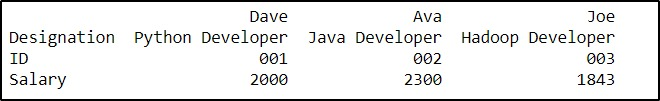
\includegraphics[scale=0.3]{figures/output}
    \caption{\textit{Output Dictionary}}
    \label{colab6}
\end{figure}
\end{lstlisting}


